%%%%%%%%%%%%%%%%%%%%%%%%%%%%%%%%%%%%%%%%%
% Journal Article
% LaTeX Template
% Version 1.3 (9/9/13)
%
% This template has been downloaded from:
% http://www.LaTeXTemplates.com
%
% Original author:
% Frits Wenneker (http://www.howtotex.com)
%
% License:
% CC BY-NC-SA 3.0 (http://creativecommons.org/licenses/by-nc-sa/3.0/)
%
%%%%%%%%%%%%%%%%%%%%%%%%%%%%%%%%%%%%%%%%%
%----------------------------------------------------------------------------------------
%    PACKAGES AND OTHER DOCUMENT CONFIGURATIONS
%----------------------------------------------------------------------------------------
\documentclass{article}
\usepackage[francais]{babel} % English language/hyphenation
\usepackage{amsmath,amsfonts,amsthm} % Math packages
\usepackage[utf8]{inputenc}
\usepackage{float}
\usepackage{amsmath}
\usepackage{mathtools}
\usepackage{blindtext}
\usepackage{graphicx} 
\usepackage{caption}
\usepackage[justification=centering]{caption} %centered caption
\usepackage{subcaption}
\usepackage{titlesec}
\setcounter{secnumdepth}{4}
\usepackage{multirow}
\usepackage{slashbox}
\usepackage{pict2e}
\usepackage{diagbox}
\usepackage[sc]{mathpazo} % Use the Palatino font
\usepackage[T1]{fontenc} % Use 8-bit encoding that has 256 glyphs
\linespread{1.05} % Line spacing - Palatino needs more space between lines
\usepackage{listings} % insert code
\usepackage{subcaption}
\usepackage{tabto}% \tab command
\usepackage{microtype} % Slightly tweak font spacing for aesthetics
\usepackage[hmarginratio=1:1,top=32mm,columnsep=20pt]{geometry} % Document margins
%\usepackage{multicol} % Used for the two-column layout of the document
%\usepackage[hang, small,labelfont=bf,up,textfont=it,up]{caption} % Custom captions under/above floats in tables or figures
%\usepackage{booktabs} % Horizontal rules in tables
\usepackage{float} % Required for tables and figures in the multi-column environment - they need to be placed in specific locations with the [H] (e.g. \begin{table}[H])
\usepackage{hyperref} % For hyperlinks in the PDF
\usepackage{lettrine} % The lettrine is the first enlarged letter at the beginning of the text
\usepackage{paralist} % Used for the compactitem environment which makes bullet points with less space between them
\usepackage{abstract} % Allows abstract customization
\renewcommand{\abstractnamefont}{\normalfont\bfseries} % Set the "Abstract" text to bold
\renewcommand{\abstracttextfont}{\normalfont\small\itshape} % Set the abstract itself to small italic text
\usepackage{titlesec} % Allows customization of titles

\titleclass{\subsubsubsection}{straight}[\subsection]
\newcounter{subsubsubsection}[subsubsection]

\renewcommand\thesubsubsubsection{\thesubsubsection.\arabic{subsubsubsection}}
\renewcommand\theparagraph{\thesubsubsubsection.\arabic{paragraph}}
\renewcommand\thesubparagraph{\theparagraph.\arabic{subparagraph}}
%\renewcommand\thesection{\Roman{section}} % Roman numerals for the sections
%\renewcommand\thesubsection{\Roman{subsection}} % Roman numerals for subsections

%\titleformat{\section}[block]{\large\scshape}{\thesection.}{1em}{} % Change the look of the section titles
%\titleformat{\subsection}[block]{\large}{\thesubsection.}{1em}{} % Change the look of the section titles

%\usepackage{pageno}
\usepackage{graphics}% resize tabular
\newcommand\scalemath[2]{\scalebox{#1}{\mbox{\ensuremath{\displaystyle #2}}}} %resize matrix
\usepackage{adjustbox}% resize code lstlisting

\usepackage{fancyhdr} % Headers and footers
\pagestyle{fancy} % All pages have headers and footers
\fancyhead{} % Blank out the default header
\fancyfoot[C]{\thepage} % Blank out the default footer

\fancyhead[C]{Université de Technologie de Compiègne $\bullet$ SY09 $\bullet$ P17} 
%%%%%%%%%%% Custom header text


\usepackage{color}
\definecolor{dkgreen}{rgb}{0,0.6,0}
\definecolor{gray}{rgb}{0.5,0.5,0.5}
\definecolor{mauve}{rgb}{0.58,0,0.82}
\lstset{ %
  language=R,                     % the language of the code
  basicstyle=\footnotesize,       % the size of the fonts that are used for the code
  numbers=left,                   % where to put the line-numbers
  numberstyle=\tiny\color{gray},  % the style that is used for the line-numbers
  stepnumber=1,                   % the step between two line-numbers. If it's 1, each line
                                  % will be numbered
  numbersep=5pt,                  % how far the line-numbers are from the code
  backgroundcolor=\color{white},  % choose the background color. You must add \usepackage{color}
  showspaces=false,               % show spaces adding particular underscores
  showstringspaces=false,         % underline spaces within strings
  showtabs=false,                 % show tabs within strings adding particular underscores
  frame=single,                   % adds a frame around the code
  rulecolor=\color{black},        % if not set, the frame-color may be changed on line-breaks within not-black text (e.g. commens (green here))
  tabsize=2,                      % sets default tabsize to 2 spaces
  captionpos=b,                   % sets the caption-position to bottom
  breaklines=true,                % sets automatic line breaking
  breakatwhitespace=false,        % sets if automatic breaks should only happen at whitespace
  title=\lstname,                 % show the filename of files included with \lstinputlisting;
                                  % also try caption instead of title
  keywordstyle=\color{blue},      % keyword style
  commentstyle=\color{dkgreen},   % comment style
  stringstyle=\color{mauve},      % string literal style
  escapeinside={\%*}{*)},         % if you want to add a comment within your code
  morekeywords={*,...}            % if you want to add more keywords to the set
} 

%----------------------------------------------------------------------------------------
%    TITLE SECTION
%----------------------------------------------------------------------------------------
% \title{\vspace{-12mm}\fontsize{24pt}{10pt}\selectfont\textbf{Discrimination}} % Article title
% \author{
% \large
% {\textsc{Yanqing ZENG~ GI05}}\\
% {\textsc{Minh Tri LÊ GI02}}
% }



%%%%%%%%%%%%%%%%%%%

\usepackage{palatino} % Use the Palatino font by default
\RequirePackage{geometry}
\geometry{
	headheight=4ex,
	includehead,
	includefoot
}
\geometry{
	paper=a4paper, % Change to letterpaper for US letter
	inner=2.5cm, % Inner margin
	outer=3.8cm, % Outer margin
	bindingoffset=.5cm, % Binding offset
	top=1.5cm, % Top margin
	bottom=1.5cm, % Bottom margin
	%showframe, % Uncomment to show how the type block is set on the page
}






%%%%%%ù


%----------------------------------------------------------------------------------------
\begin{document}



\begin{titlepage}

\newcommand{\HRule}{\rule{\linewidth}{0.5mm}} % Defines a new command for the horizontal lines, change thickness here

\center % Center everything on the page
 
%----------------------------------------------------------------------------------------
%	HEADING SECTIONS
%----------------------------------------------------------------------------------------

\textsc{\LARGE Université de Technologie de Compiègne}\\[1.5cm] % Name of your university/college
\textsc{\Large Rapport TP4 SY09}\\[0.5cm] % Major heading such as course name
%\textsc{\large Étude expérimentale}\\[0.5cm] % Minor heading such as course title

%----------------------------------------------------------------------------------------
%	TITLE SECTION
%----------------------------------------------------------------------------------------

\HRule \\[0.4cm]
{ \huge \bfseries Discrimination}\\[0.4cm] % Title of your document
\HRule \\[1.5cm]
 
%----------------------------------------------------------------------------------------
%	AUTHOR SECTION
%----------------------------------------------------------------------------------------

\begin{minipage}{0.4\textwidth}
\begin{flushleft} \large
%\emph{Étudiant :}\\
Minh Tri \textsc{Lê} GI02 % Your name
\end{flushleft}
\end{minipage}
~
\begin{minipage}{0.4\textwidth}
\begin{flushright} \large
%\emph{Suivi par :} \\
Yanqing \textsc{ZENG} GI05% Supervisor's Name
\\
\end{flushright}
\end{minipage}\\[2cm]


%----------------------------------------------------------------------------------------
%	DATE SECTION
%----------------------------------------------------------------------------------------

{\large \today}\\[2cm] % Date, change the \today to a set date if you want to be precise

%----------------------------------------------------------------------------------------
%	LOGO SECTION
%----------------------------------------------------------------------------------------

\includegraphics[scale=0.1]{logo_utc.jpg}\\[1cm] % Include a department/university logo - this will require the graphicx package
 
%----------------------------------------------------------------------------------------

\vfill % Fill the rest of the page with whitespace

\end{titlepage}




%\maketitle % Insert title
\thispagestyle{fancy} % All pages have headers and footers



\tableofcontents

\listoffigures
\listoftables

\newpage

\section*{Introduction}

Les objectifs de ce TP sont d'une part d'étudier diverses méthodes de classifieurs sur différents jeux de données afin d'en comparer les performances. D'autre part, de pouvoir interpréter les résultats obtenus afin d'être capable de choisir le classifieur le plus adapté aux problème par la suite.


\section{Programmation}

Le code des 3 modèles d'analyse discriminante, ainsi que la fonction effectuant les prédictions en fonction des paramètres [\ref{ad.val}] sont fournis en annexe.



\subsection{Analyse discriminante}
Nous ferons quelques rappels sur les hypothèses et les estimateurs spécifiques à chaque méthode (Analyse discriminaten quadratique, analyse discriminante linéaire, classifieur bayésien naïf).

% Mettre code 4 fonctions en annexe

% Mettre les estimateurs prop, mu, sigma, de chaque algorithmes

Pour les 3 classifieurs, on émet l'hypothèse suivante :
La matrice X suit conditionnellement à chaque classe $w_k$ une loi normale multidimensionnelle d'espérance $\mu_k$ et de variance $\sum_k$.
\medskip

Chaque classifieur se différencie d'un autre en fonction des hypothèses faites sur les paramètres de la loi normale.

La loi normale multidimensionnelle pour chaque classe $k$ s'énonce comme-ci :
\[f_k(x)=\frac{1}{(2\pi)^{p/2}(det \sum_k)^{\frac{1}{2}}}~
exp \left( -   \frac{1}{2} ( (x-\mu_k)^T)\sum_k^-1 (x-\mu_k) \right)
\]

La règle de Bayes s'écrit alors :
\[
\delta^*(x)=arg~ \underset{k}{max}~ P(w_k|x)
\]

Avec 
\[
P(w_k|k)=\frac{\pi_k f_k(x)}{f(x)}
\]
(pour $g=2$ classes)
\[=
P(w_k|k)=\frac{\pi_k f_k(x)}{\pi_1 f_1(x)) + \pi_2 f_2(x)}
\]

\subsection{Analyse discrimante quadratique}

L'analyse discriminante quadratique considère le cas général : La distribution des variables dans chaque classe est caractérisée par des $\mu_k$ et $\sum_k$ différents.

Pour l'estimation des paramètres, nous avons choisi les estimateurs sans biais pour la proportion $ \widehat{\pi_k},  \widehat{\mu_k}  \widehat{\sum_k}  $
\[
 \widehat{\pi_k} = \frac{n_k}{n},
\]
\[
  \widehat{\mu_k} = \overline{x_k}=\frac{1}{n_k}\sum_{i=1}^{n} z_{ik}x_i,
  \]
  \[
   \widehat{\Sigma_k^*} = V_k^* = \frac{n_k}{n_k-1}V_k
\]
avec
  \[
   V_k^* = \frac{1}{n_k}\sum_{i=1}^{n} z_{ik}(x_i-\widehat{\mu_k})(x_i-\widehat{\mu_k})^T
\]

Le code est en annexe \ref{adq.val}.


\subsection{Analyse discrimante linéaire}

L'analyse discriminante linéaire considère que la variance est commune à toutes les classes (hypothèse d'homoscédasticité) : $\Sigma_k=\Sigma,~ k \in \lbrace1, ...., g\rbrace$. 
\medskip

De plus, l'estimation de $\widehat{\pi_k}$ et $\widehat{\mu_k}$ est identique aux paramètres de l'analyse discrimnante linéaire.
\smallskip

Nous avons choisi les estimateurs sans biais pour la variance $ \widehat{\sum_k}  $ :

  \[
   V_W^* =\frac{1}{n-g} \sum_{k=1}^g (n_k-1) V_k^*
\]

Le code est en annexe \ref{adl.val}.

\subsection{Classifieur bayésien naïf}

Classifieur bayésien naïf considère que les variables $X_j$ sont indépendantes entre-elles conditionnellement à $Z$, ce qui revient à supposer que les matrices de variance $\sum_k$ sont diagonales.
\medskip

De plus, les estimations de $\pi_k$ et $\mu_k$ sont les mêmes que précedemment.

Pour la variance, on a :
  \[
   \widehat{\Sigma_k} = diag(s_{k1}^2, ...., s_{kj}^2, ...., s_{kp}^2)
\]
 \[
   \widehat{\Sigma_k^*} = diag(V_k)
\]

Le code est en annexe \ref{nba.app}.











\subsection{Régression logistique}
La méthode de régression logistique consiste à modéliser les probabilités à posteriori $P( w_k | x )$ par des fonctions de x.
Dans ce TP, nous appliquons la fonction logit, qui est le logarithme du rapport des probabilité a posteriori $P(k_k | x)$ et $P(w_g|x )$.
\[
	ln\frac{P(w_k|x)}{P(w_g|x)}=w_k^Tx
\]
Pour estimer les valeurs de composantes de $w$, on va maximiser la vraisemblance :
\[
logL(w;t_1,t_2,......,t_n)=\sum_{i=1}^{n}(t_iW^Tx_i-log(1+exp(w^Tx_i)))
\]
Le gradient est donc :
\[
\frac{\delta logL(w)}{\delta w}=X^T(t-p)
\]
On cherche donc les paramètres tels que :
\[
X^T(t-p)=0
\]
On ne peut pas résoudre ce système directement, donc on utilise : l'algorithme de Newton Raphson pour trouver des valeurs qui approchent la solution optimale locale par itération successive.
\[
w^{(k+1)}=w^{(q)}+(X^TW_{(q)}X)^{-1}X^T(t-p^{(q)})
\]

Enfin, notre fonction de régression logistique admet une variable booléenne pour l'ajout ou non d'une ordonnée à l'origine aux vecteurs $x_i$ d'individus. Cela permet d'ajout une dimension à notre frontière de décision et ajoute de la flexibilité au classifieur.\\
Dans ce TP nous tenterons de si cet ajout est pertinent pour la prédiction de nos jeux de données.



Le code est en annexe \ref{log.app}.

Pour la méthode de régression logistique quadratique, on a construit la matrice quadratique par la fonction quadratique(X), le code est en annexe \ref{quadratique}. La régression logistique quadratique est plus flexible mais nécessite d'estimer un nombre de paramètres plus important ($\frac{p(p+3)}{2}$).


\subsection{Vérification des fonctions}

\begin{figure}[H]   
  \begin{minipage}[t]{0.5\linewidth} 
    \centering   
    \includegraphics[width=6cm]{img/adl.png}   
    \caption{Vérification : adl.app}   
    \label{veri_adl}   
  \end{minipage}%   
  \begin{minipage}[t]{0.5\linewidth}   
    \centering   
    \includegraphics[width=6cm]{img/adq.png}   
    \caption{Vérification : adq.app}   
    \label{veri_adq}   
  \end{minipage}   
\end{figure}
\begin{figure}[H]
\centering
\includegraphics[width=6cm]{img/nba.png}
\caption{Vérification : nba.app}
\end{figure}
\begin{figure}[H]   
  \begin{minipage}[t]{0.5\linewidth} 
    \centering   
    \includegraphics[width=6cm]{img/log1.png}   
    \caption{Vérification : logistique}   
    \label{veri_log1}   
  \end{minipage}%   
  \begin{minipage}[t]{0.5\linewidth}   
    \centering   
    \includegraphics[width=6cm]{img/log2.png}   
    \caption{Vérification : logistique quadratique}
    \label{veri_log2}   
  \end{minipage}   
\end{figure}  








\section{Application}




\subsection{Test sur des données simulées}
On a appliqué la méthode de analyse discriminante quadratique, linéaire, classifieur bayésien naif et la méthode de régression logistique (et quadratique) sur les jeux de données simulées, qui suivent une distribution gaussienne.

Au point de vue de la complexité temporelle, nous avons constaté que la méthode de l'arbre de décision est la moins coûteuse, car c'est un modèle non paramétrisé. Il a la variance la plus élevé, car il se concentre plus sur les individus, et le modèle varie beaucoup selon la partition des données faite.
% SynthN-1000
\subsubsection{Synth1-1000}

\begin{table}[H]
\centering
\caption{Calcul du taux d'erreur d'apprentissage $\varepsilon$ et de test pour le jeu de données Synth1-1000 avec plusieurs méthodes (arrondi à $10^{-4})$}
\begin{tabular}{l|l|cc}
\multicolumn{1}{l|}{\textbf{Méthode}}    & \textbf{Données} &$ \overline{\varepsilon}$ & $IC$                      \\ \hline
\multirow{2}{*}{Analyse discriminante quadratique} & Apprentissage    & 0.0312                   & $\left[0.0228 ;~ 0.0395 \right]$  \\
                                       & Test             & 0.0310             & $\left[0.0192  ;~ 0.0428 \right]$ \\ \hline
\multirow{2}{*}{Analyse discriminante linéaire}                  & Apprentissage & 0.0420                                 & $\left[0.0346 ;~ 0.0494 \right]$  \\
                                       & Test             & 0.0455                       & $\left[0.0309  ;~ 0.0601 \right]$ \\ \hline
\multirow{2}{*}{Classifieur bayésien naïf}                  & Apprentissage    & 0.0419                             & $\left[0.0338 ;~ 0.0500 \right]$  \\
                                       & Test             & 0.0436                                 & $\left[0.0236 ;~ 0.0636 \right]$ \\ \hline
\multirow{2}{*}{Régression logistique (intercept=1)}                  & Apprentissage    & 0.0327                             & $\left[0.0235 ;~ 0.0419 \right]$  \\
                                       & Test             & 0.0325                                 & $\left[0.0183;~ 0.0466 \right]$ \\ \hline
\multirow{2}{*}{Régression logistique (intercept=0)}                  & Apprentissage    & 0.0417                           & $\left[0.0334 ;~ 0.0501\right]$  \\
                                       & Test             & 0.0412                                & $\left[0.0277 ;~ 0.0546 \right]$ \\ \hline
\multirow{2}{*}{Régression logistique quadratique (intercept=1)}                  & Apprentissage    & 0.0312                            & $\left[0.0203 ;~ 0.0420 \right]$  \\
                                       & Test             & 0.0356                                & $\left[0.0215;~ 0.0497 \right]$ \\ \hline
\multirow{2}{*}{Régression logistique quadratique (intercept=0)}                  & Apprentissage    & 0.0420                            & $\left[0.0342 ;~ 0.0498\right]$  \\
                                       & Test             & 0.0425                                 & $\left[0.0252 ;~ 0.0598 \right]$ \\ \hline      
\multirow{2}{*}{Arbre de décision}                  & Apprentissage    & 0.0261                             & $\left[0.0172 ;~  0.0349 \right]$  \\
                                       & Test             & 0.0485                                 & $\left[0.0259 ;~ 0.0711 \right]$ 
\end{tabular}


\label{err_1-1000}
\end{table}









\subsubsection{Synth2-1000}

\begin{table}[H]
\centering
\caption{Calcul du taux d'erreur d'apprentissage $\varepsilon$ et de test pour le jeu de données Synth2-1000 avec plusieurs méthodes (arrondi à $10^{-4})$}
\begin{tabular}{l|l|cc}
\multicolumn{1}{l|}{\textbf{Méthode}}    & \textbf{Données} &$ \overline{\varepsilon}$ & $IC$                      \\ \hline
\multirow{2}{*}{Analyse discriminante quadratique} & Apprentissage    & 0.0603                   & $\left[0.0519 ;~ 0.0688 \right]$  \\
                                       & Test             & 0.0602             & $\left[0.0448  ;~ 0.0757 \right]$ \\ \hline
\multirow{2}{*}{Analyse discriminante linéaire}                  & Apprentissage & 0.0805                                & $\left[0.0662 ;~ 0.0948 \right]$  \\
                                       & Test             & 0.0824                      & $\left[0.0633  ;~ 0.1016 \right]$ \\ \hline
\multirow{2}{*}{Classifieur bayésien naïf}                  & Apprentissage    & 0.0615                            & $\left[0.0504 ;~ 0.0725 \right]$  \\
                                       & Test             & 0.0650                                & $\left[ 0.0503 ;~ 0.0797 \right]$ \\ \hline
\multirow{2}{*}{Régression logistique (intercept=1)}                  & Apprentissage    & 0.0690                           & $\left[0.0551 ;~ 0.0829 \right]$  \\
                                       & Test             & 0.0731                                 & $\left[0.0548;~ 0.0915 \right]$ \\ \hline
\multirow{2}{*}{Régression logistique (intercept=0)}                  & Apprentissage    & 0.0720                             & $\left[0.0555 ;~ 0.0885\right]$  \\
                                       & Test             & 0.0763                                 & $\left[0.0473 ;~ 0.1053 \right]$ \\ \hline
\multirow{2}{*}{Régression logistique quadratique (intercept=1)}                  & Apprentissage    & 0.0619                             & $\left[0.0492 ;~ 0.0747 \right]$  \\
                                       & Test             & 0.0643                                 & $\left[0.0399;~ 0.0887 \right]$ \\ \hline
\multirow{2}{*}{Régression logistique quadratique (intercept=0)}                  & Apprentissage    & 0.0614                             & $\left[0.0515 ;~ 0.0765\right]$  \\
                                       & Test             & 0.0669                                 & $\left[0.0565 ;~ 0.0774 \right]$ \\ \hline      
\multirow{2}{*}{Arbre de décision}                  & Apprentissage    & 0.0445                             & $\left[0.0304 ;~ 0.0587 \right]$  \\
                                       & Test             & 0.07808                                & $\left[0.0552 ;~ 0.1009 \right]$ 
\end{tabular}


\label{err_2-1000}
\end{table}









\subsubsection{Synth3-1000}

\begin{table}[H]
\centering
\caption{Calcul du taux d'erreur d'apprentissage $\varepsilon$ et de test pour le jeu de données Synth3-1000 avec plusieurs méthodes (arrondi à $10^{-4})$}
\begin{tabular}{l|l|cc}
\multicolumn{1}{l|}{\textbf{Méthode}}    & \textbf{Données} &$ \overline{\varepsilon}$ & $IC$                      \\ \hline
\multirow{2}{*}{Analyse discriminante quadratique} & Apprentissage    & 0.0628                   & $\left[0.0528 ;~ 0.0728 \right]$  \\
                                       & Test             & 0.0656            & $\left[ 0.0450  ;~ 0.0862 \right]$ \\ \hline
\multirow{2}{*}{Analyse discriminante linéaire}                  & Apprentissage & 0.0795                               & $\left[0.0657 ;~ 0.0933 \right]$  \\
                                       & Test             &  0.0827                     & $\left[0.0567  ;~ 0.1087 \right]$ \\ \hline
\multirow{2}{*}{Classifieur bayésien naïf}                  & Apprentissage    & 0.0646                           & $\left[0.0526 ;~ 0.0766 \right]$  \\
                                       & Test             & 0.0662                             & $\left[ 0.0521 ;~ 0.0803 \right]$ \\ \hline
\multirow{2}{*}{Régression logistique (intercept=1)}                  & Apprentissage    & 0.0410                            & $\left[0.0355;~ 0.0465 \right]$  \\
                                       & Test             &0.0390                                & $\left[0.0212;~ 0.0569 \right]$ \\ \hline
\multirow{2}{*}{Régression logistique (intercept=0)}                  & Apprentissage    & 0.0403                            & $\left[0.0296 ;~ 0.0511\right]$  \\
                                       & Test             & 0.0393                                 & $\left[0.0257 ;~ 0.0530 \right]$ \\ \hline
\multirow{2}{*}{Régression logistique quadratique (intercept=1)}                  & Apprentissage    & 0.0396                            & $\left[0.0297 ;~ 0.0494 \right]$  \\
                                       & Test             & 0.0410                                & $\left[0.0223;~ 0.0597 \right]$ \\ \hline
\multirow{2}{*}{Régression logistique quadratique (intercept=0)}                  & Apprentissage    & 0.0395                             & $\left[0.0303 ;~ 0.0487\right]$  \\
                                       & Test             & 0.0362                                 & $\left[0.0242 ;~ 0.0482 \right]$ \\ \hline      
\multirow{2}{*}{Arbre de décision}                  & Apprentissage    & 0.0362                            & $\left[ 0.0234;~ 0.0490 \right]$  \\
                                       & Test             & 0.0611                                 & $\left[0.0308 ;~ 0.0914 \right]$ 
\end{tabular}


\label{err_3-1000}
\end{table}
\textbf{Interprétation }: Pour tous les jeux de données simulées (Synth-\textit{n}), tous les classifieurs ont un taux d'erreur très bas.

La méthode discrimiante quadratique et la régression logistique quadratique avec intercept=1 ont la meilleure performance. Les paramètres à estimer pour ces deux méthodes sont les plus importantes, donc ces modèles ont plus de flexibilité que les autres.

En effet, les modèles analyse discriminante linéaire et classifieur bayésien naïf sont des modèles plus simplifiés. On peut donc appliquer ces deux méthodes si on ne veut pas avoir un fort coût de la complexité temporelle, comme il y a moins de paramètres à estimer.

Plus généralement, les classifieurs se basant sur la distribution gaussienne ont de très bons résultats sur ces données car cela correspond effectivement à la vraie distribution des données.




\subsection{Test sur des données réelles}

Pour calculer le taux d'erreur ponctuelle $ \widehat{\varepsilon}$ d'une prédiction, il faut simplement compter le nombre de prédictions erronées $\varepsilon_{i}$ entre la prédiction faite et les données réelles (d'apprentissage ou de test), puis diviser par le nombre total d'individus $n$.

On répète cette procédure \textit{N} fois pour obtenir \textit{N} réalisations du taux d'erreur.
Pour obtenir l'estimation du taux d'erreur $ \overline{\varepsilon}$, il ne reste plus qu'à faire la moyenne des N réalisations.\\
L'intervalle de confiance à $95\%$ est obtenu comme-ci : $IC= \left[ \mu -1.96* \frac{s^*}{\sqrt{N} } ;~  \mu +1.96* \frac{s^*}{\sqrt{N} }   \right]$. 

Avec : 
\begin{itemize}
\item $\mu$ : La moyenne des $N$ réalisations de $\varepsilon$
\item $s^*$ : L'écart-type corrigé des $N$ réalisations de $\varepsilon$
\item $N$ : Le nombre de réalisations de $\varepsilon$
\end{itemize}


\subsubsection{Pima}
Nous avons appliqué les différents modèles d'analyses discriminantes, de régression logistique ainsi que les arbres de décision.

Pour calculer le taux d'erreur sur les modèles d'analyse discriminantes, nous avons choisi d'effectuer $N=100$ répétitions pour calculer le taux d'erreur et son intervalle de confiance (à $96\%$). Le résumé des résultats sont en table \ref{err_pima}.


\begin{table}[H]
\centering
\caption{Calcul du taux d'erreur d'apprentissage $\varepsilon$ et de test pour le jeu de données Pima avec plusieurs méthodes (arrondi à $10^{-4})$}
\begin{tabular}{l|l|cc}
\multicolumn{1}{l|}{\textbf{Méthode}}    & \textbf{Données} &$ \overline{\varepsilon}$ & $IC$                      \\ \hline
\multirow{2}{*}{Analyse discriminante quadratique} & Apprentissage    & 0.2135                   & $\left[0.2105 ;~ 0.2165 \right]$  \\
                                       & Test             & 0.2385             & $\left[0.2332  ;~ 0.2438 \right]$ \\ \hline
\multirow{2}{*}{Analyse discriminante linéaire}                  & Apprentissage & 0.2096                                 & $\left[0.2070 ;~ 0.2122 \right]$  \\
                                       & Test             & 0.2233                       & $\left[0.2172  ;~ 0.2273 \right]$ \\ \hline
\multirow{2}{*}{Classifieur bayésien naïf}                  & Apprentissage    & 0.2291                             & $\left[0.2268 ;~ 0.2314 \right]$  \\
                                       & Test             & 0.2363                                 & $\left[0.2307 ;~ 0.2420 \right]$ \\ \hline
\multirow{2}{*}{Régression logistique (intercept=1)}                  & Apprentissage    & 0.2090                             & $\left[0.2069 ;~ 0.2111 \right]$  \\
                                       & Test             & 0.2196                                 & $\left[0.2149 ;~ 0.2244 \right]$ \\ \hline
\multirow{2}{*}{Régression logistique (intercept=0)}                  & Apprentissage    & 0.2759                             & $\left[0.2735 ;~ 0.2783 \right]$  \\
                                       & Test             & 0.2853                                 & $\left[0.2807 ;~ 0.2899 \right]$ \\ \hline
\multirow{2}{*}{Régression logistique quadratique (intercept=1)}                  & Apprentissage    & 0.1861                             & $\left[0.1832 ;~ 0.1890 \right]$  \\
                                       & Test             & 0.2459                                 & $\left[0.2411 ;~ 0.2508 \right]$ \\ \hline
\multirow{2}{*}{Régression logistique quadratique (intercept=0)}                  & Apprentissage    & 0.1871                             & $\left[0.1843 ;~ 0.1899 \right]$  \\
                                       & Test             & 0.2407                                 & $\left[0.2360 ;~ 0.2454 \right]$ \\ \hline                                       
\multirow{2}{*}{Arbre de décision}                  & Apprentissage    & 0.1958                             & $\left[0.1856 ;~ 0.2019 \right]$  \\
                                       & Test             & 0.2429                                 & $\left[0.2374 ;~ 0.2485 \right]$ 
\end{tabular}


\label{err_pima}
\end{table}

D'après \ref{err_pima}, parmi les trois méthodes discriminantes, l'analyse discriminante linéaire permet d'obtenir les meilleurs résultats, suivi de près par le classifieur bayésien et l'analyse discriminante quadratique.\\
Nous pouvons expliquer cela par le fait que le modèle linéaire comporte moins de paramètres que le modèle quadratique donc il est plus général et plus robuste sur de nouvelles données. En revanche, le classifieur bayésien possède le moins de paramètres et n'est donc pas assez flexible pour ce jeu de données.

La régression logistique (avec l'ajout d'une ordonnée à l'origine) permet d'obtenir le plus faible taux d'erreur. Tandis que la régression logistique (sans l'ajout d'une ordonnée à l'origine) obtient le taux d'erreur le plus fort.\\
On constate donc que l'ajout de l'ordonnée à l'origine est un paramètre à considérer pour la régression logistique car l'écart de résultat est net.

De manière plus générale, la performance des prédictions obtenues avec toutes nos méthodes est nettement moins effective que pour les données simulées. Nous pouvons donc supposer que les variables décrivant les individus de \textit{pima} ne suivent pas une loi normale multidimensionnelle. Ce qui pourrait expliquer la performance moyenne des modèles faisant cette hypothèse.


\subsubsection{Breast cancer Wisconsin}

Comme pour le précédent jeu de données, nous appliquons les mêmes méthodes de prédiction (sauf la régression logistique quadratique) avec $N=100$ répétitions.

\begin{table}[H]
\caption{Calcul du taux d'erreur d'apprentissage $\varepsilon$ et de test pour le jeu de données BCW avec plusieurs méthodes (arrondi à $10^{-4})$}
\centering

\begin{tabular}{l|l|cc}
\multicolumn{1}{l|}{\textbf{Méthode}}    & \textbf{Données} &$ \overline{\varepsilon}$ & $IC$                      \\ \hline
\multirow{2}{*}{Analyse discriminante quadratique} & Apprentissage    & 0.0437                                 & $\left[0.0426 ;~ 0.0448 \right]$  \\
                                       & Test             & 0.0522                                 & $\left[0.0499  ;~ 0.0546 \right]$ \\ \hline
\multirow{2}{*}{Analyse discriminante linéaire}                  & Apprentissage    & 0.0389                             & $\left[0.0378 ;~ 0.0401 \right]$  \\
                                       & Test             & 0.0450                       & $\left[0.0427 ;~ 0.0473 \right]$ \\ \hline
\multirow{2}{*}{Classifieur bayésien naïf}                  & Apprentissage    & 0.0368             & $\left[0.0356 ;~ 0.0380 \right]$  \\
                                       & Test             & 0.0384                                 & $\left[0.0366 ;~ 0.0407 \right]$ \\ \hline
\multirow{2}{*}{Régression logistique (intercept=1)}                  & Apprentissage    & 0.0383                             & $\left[0.0371 ;~ 0.0395 \right]$  \\
                                       & Test             & 0.0465                                 & $\left[0.0443;~ 0.0487 \right]$ \\ \hline
\multirow{2}{*}{Régression logistique (intercept=0)}                  & Apprentissage    & 0.1444                             & $\left[0.1424 ;~ 0.1464\right]$  \\
                                       & Test             & 0.1574                                 & $\left[0.1534 ;~ 0.1613 \right]$ \\ \hline

\multirow{2}{*}{Arbre de décision}                  & Apprentissage    & 0.0312                             & $\left[0.0292 ;~ 0.0332 \right]$  \\
                                       & Test             & 0.0579                                 & $\left[0.0548 ;~ 0.0609 \right]$ 
\end{tabular}


\label{err_bcw}
\end{table}

D'après la table \ref{err_bcw}, le classifieur bayésien naïf permet d'obtenir les meilleurs résultats, alors que la régression logistique (sans l'ajout de l'ordonnée à l'origine) obtient une fois encore le taux d'erreur le plus fort.\\

L'écart de performance entre l'ajout ou non de l'ordonnée à l'origine est très marqué pour la régression logistique. Cela confirme donc que c'est un paramètre important à prendre en compte.

Parmi les trois méthodes discriminantes, le taux d'erreur augmente quand le nombre de paramètre est plus important (le modèle linéaire obtient de meilleurs résultats que le modèle quadratique qui a plus de paramètres.)

De manière plus générale, la performance des prédictions obtenues avec toutes nos méthodes est très effective. Nous pouvons donc supposer que les variables décrivant les individus de \textit{pima} suivent une loi normale multidimensionnelle. Ce qui explique la bonne performance des modèles faisant cette hypothèse. 

Enfin, il s'avère qu'un modèle générale et donc avec peu de paramètres est le plus adapté à ce jeu de données.











\section{Challenge : Spam}

Ce jeu de données comporte 58 variables pour 4601 individus. 
On a exclu la première colonne, car cela correspond à l'index qui est inutile pour notre analyse.

\subsection{L'arbre de décision}
Nous avons tout d'abord tenté la méthode de l'arbre de décision, car cela nous permet d'effectuer une classification générale avec un coût temporel peu important. En plus, cette méthode minimise l'impureté à chaque itération, donc on peut obtenir un modèle convenable sans prétraitement de données.

\begin{figure}[H]
\centering
\includegraphics[width=8cm]{img/arbre_spam.png}
\caption{La classification de spam avec l'arbre de décision}
\label{arbre_spam}
\end{figure}
On a effectué N=100 répétitions, et on obtient $ \overline{\varepsilon}=0.0867$, avec $sd=0.0086$ et $IC=\left[0.0698,0.1035\right]$

\subsection{L'analyse discriminante}

Nous mettons ensuite à l'essai les modèles d'analyse discriminante.

Pour l'analyse discriminante linéaire, nous n'avons effectué aucun pré-traitement de données avec $N=100$ répétitions.
\begin{table}[H]
\centering
\caption{Calcul du taux d'erreur d'apprentissage $\varepsilon$ et de test pour le jeu de données \textit{Spam} avec l'analyse discriminante linéaire (arrondi à $10^{-4})$}
\begin{tabular}{l|l|cc}
\multicolumn{1}{l|}{\textbf{Méthode}}    & \textbf{Données} &$ \overline{\varepsilon}$ & $IC$                      \\ \hline
\multirow{2}{*}{Analyse discriminante linéaire}                  & Apprentissage    & 0.1132                             & $\left[0.1123 ;~ 0.1141 \right]$  \\
                                       & Test             & 0.1172                                 & $\left[0.1156 ;~ 0.1188 \right]$ \\ 
\end{tabular}

\label{spam_adl}
\end{table}

En revanche, pour l'analyse discriminante quadratique et le classifieur bayésien, nous avons rencontré des difficultés. La matrice de variance contient des valeurs propres nulles ou très proches de 0. De ce fait, la factorisation de Cholesky sur la matrice de variance échoue. 
\begin{lstlisting}
Error in chol.default(Sigma): the leading minor of order 40 is not positive definite
\end{lstlisting}

Notons que ce problème apparaît à intermittence : il est parfois possible (selon la séparation aléatoire des données d'apprentissage), d'obtenir une prédiction. Dans ce cas, le taux d'erreur avoisine les $0.160$ pour l'analyse discriminante quadratique et $0.180$ pour le classifieur bayésien. Par expérience, nous avons observé plus d'échec dans la factorisation de Cholesky que de succès.




Pour résoudre ce problème, nous avons donc 2 solutions :
\begin{itemize}
\item Faire un centrage-réduction pour le prétraitement
\item Utiliser une méthode de sélection de variable
\end{itemize}

\subsubsection{Solution 1 : Par centrage-réduction}
Nous avons encore rencontré une erreur car la capacité mémoire a été atteinte.

\begin{lstlisting}
Error in array(0, c(p, p, g)): negative length vectors are not allowed
Traceback:

1. run_test(spam_sc[, 2:ncol(spam_sc)], nba.app, 1)
2. func(Xapp, zapp)   # at line 32 of file <text>
3. array(0, c(p, p, g))   # at line 110 of file <text>
\end{lstlisting}

Cela correspond à cette ligne de la fonction nba.app :
\begin{lstlisting}
param$MCov <- array(0, c(p,p,g))
\end{lstlisting}
lors de la création de l'array multi-dimensionnel de la matrice de covariance.
Le problème est identique pour adq.app, le besoin mémoire est trop important pour ce jeu de données.

Nous ne pouvons donc pas utiliser le centrage-réduction.

\subsubsection{Solution 2 : Par sélection de variable}
Les méthodes de sélection de variables n'est pas au programme de SY09. 

En revanche, nous pouvons utiliser l'ACP (analyse en composante principale), comme vu au premier et second TP. C'est une méthode de sélection de variable assez naïve et moins efficace que les méthodes traditionnelles.

En effectuant un centrage-réduction puis l'ACP, nous obtenons les pourcentage d'inertie expliquée suivants : \ref{acp_eigen}

\begin{figure}[H]
\centering   
    \includegraphics[width=15cm]{img/acp_eigen_percent.PNG}   
    \caption{Pourcentage d'inertie expliquée selon les axes factoriels}   
    \label{acp_eigen}   
    
\end{figure}
 
Les axes factoriels expliquent peu d'information, il faut prendre en compte les $45^{ème}$ premiers axes pour avoir au moins 90\% de l'inertie expliquée. (\ref{acp_eigen_cum})
 
\begin{figure}[H]
\centering   
    \includegraphics[width=15cm]{img/acp_eigen_cumul.PNG}   
    \caption{Pourcentage d'inertie expliquée cumulé selon les axes factoriels}   
    \label{acp_eigen_cum}   
    
\end{figure} 


Ensuite, en effectuant la représentation des variables (\ref{acp_var}).

\begin{figure}[H]
\centering   
    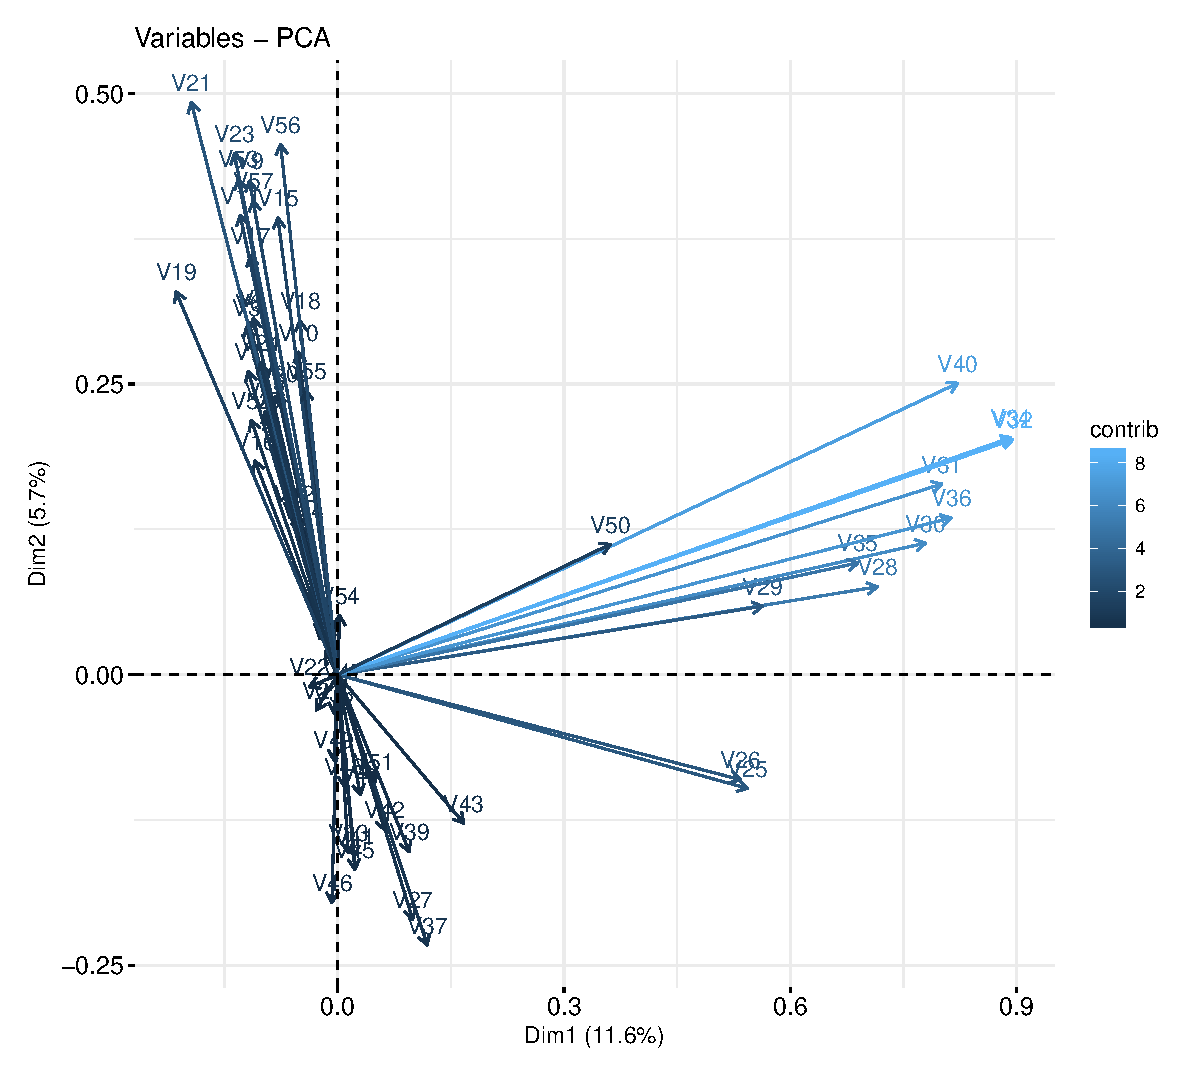
\includegraphics[scale=0.7]{img/acp_var2.eps}   
    \caption{Représentation des variables dans le premier plan factoriel}   
    \label{acp_var}   
    
\end{figure}

Nous en déduisons que la qualité de la représentation obtenues par l'ACP n'est pas très bonne car la réduction des variables n'est pas effective.

Nous décidons de tout de même appliquer l'analyse discriminante quadratique et le classifieur bayésien avec l'ACP, en tenant compte de toutes les variables.

Nous obtenons les taux d'erreurs suivants :



\begin{table}[H]
\centering
\caption{Calcul du taux d'erreur d'apprentissage $\varepsilon$ et de test pour le jeu de données \textit{Spam} avec l'analyse discriminante quadratique et le classifieur bayésien naïf, avec centrage-réduction et ACP (arrondi à $10^{-4})$}
\begin{tabular}{l|l|cc}
\multicolumn{1}{l|}{\textbf{Méthode}}    & \textbf{Données} &$ \overline{\varepsilon}$ & $IC$                      \\ \hline
\multirow{2}{*}{Analyse discriminante quadratique}                  & Apprentissage    & 0.1659                             & $\left[0.1649 ;~ 0.1669 \right]$  \\
                                       & Test             & 0.1703                                 & $\left[0.1686 ;~ 0.1720 \right]$ \\ \hline
\multirow{2}{*}{Classifieur bayésien naïf}                  & Apprentissage    & 0.2284                             & $\left[0.2257;~ 0.2311 \right]$  \\
                                       & Test             & 0.2314                                 & $\left[0.2279 ;~ 0.2349 \right]$ \\ 
\end{tabular}

\label{spam_ad}
\end{table}

Nous remarquons que l'estimation de l'erreur pour $N=100$ répétitions de l'analyse discriminante est proche de la valeur ponctuelle trouvée précédemment sans pré-traitement de données. Ce n'est pas le cas pour le classifieur bayésien où le taux d'erreur avec l'ACP est plus important que la valeur trouvée précédemment.


\subsection{Régression logistique}

Nous testons ensuite la régression logistique pour ce jeu de données, toujours avec $N=100$ répétitions.


\begin{table}[H]
\centering
\caption{Calcul du taux d'erreur d'apprentissage $\varepsilon$ et de test pour le jeu de données \textit{Spam} avec la régression logistique (arrondi à $10^{-4})$}
\begin{tabular}{l|l|cc}
\multicolumn{1}{l|}{\textbf{Méthode}}    & \textbf{Données} &$ \overline{\varepsilon}$ & $IC$                      \\ \hline
\multirow{2}{*}{Régression logistique (intercept=1)}                  & Apprentissage    & 0.1097                             & $\left[0.1088 ;~ 0.1106 \right]$  \\
                                       & Test             & 0.1125                                 & $\left[0.1113 ;~ 0.1138 \right]$ \\ \hline
\multirow{2}{*}{Régression logistique (intercept=0)}                  & Apprentissage    & 0.1064                             & $\left[0.1052 ;~ 0.1077 \right]$  \\
                                       & Test             & 0.1111                                 & $\left[0.1094 ;~ 0.1129 \right]$ \\ 
\end{tabular}

\label{spam_logit}
\end{table}

Notons qu'il n'a pas été possible d'effectuer la régression logistique quadratique car nous sommes tombés sur ce problème :
\begin{lstlisting}
Error in solve.default(tXap% * %MatW% * %Xapp): Lapack routine dgesv: system is exactly singular: U[254,254] = 0
Traceback:

1. run_test_logit_quadra(spam[, 2:ncol(spam)], log.app, 100, 1)
2. func(Xapp, zapp, orig, 1e-06)   # at line 90 of file <text>
3. solve(tXap% * %MatW% * %Xapp)   # at line 32 of file <text>
4. solve.default(tXap% * %MatW% * %Xapp)
\end{lstlisting}

En d'autre terme, à un moment donné, nous obtenons ce résultat :
\[
det(X^TW_{(q)}X)=0
\]

Par définition, il n'est donc pas possible d'inverser cette matrice. Or, on rappelle qu'il est nécessaire de calculer $(X^TW_{(q)}X)^{-1}$ pour calculer la mise à jour du vecteur de poids $w^{(q)}$ à l'itération $q+1$.





\subsection*{Conclusion sur les classifieurs pour \textit{Spam}}

Parmi nos différents classifieur, le meilleur est nettement l'arbre de décision. Derrière se place la régression logistique (avec ou sans ajout de l'origine), l'analyse discriminante linéaire puis encore après, l'analyse discriminante quadratique et enfin le classifieur bayésien naïf.

Nous pouvons donc supposer que les données \textit{spam} ne sont pas compatibles avec des modèles ayant beaucoup de paramètres (analyse discriminante quadratique) ou trop peu (classifieur bayésien naïf) et que les variables ne semblent pas suivre pas une loi normale multivariée.

\section*{Conclusion}

Cette deuxième partie sur l'apprentissage supervisé nous a permis de mettre en pratique de nombreuses méthodes de discriminations sur des jeux de données simulés et réels. \\
Nous avons donc pu être confronté aux difficultés de trouver le modèle le plus adapté au jeu de données.
En particulier, nos différents résultats souligne l'importance de bien comprendre les hypothèses faites par chaque méthode ainsi que d'avoir un bon compromis entre robustesse et flexibilité. Il faut mettre ce dernier en rapport avec la quantité de données disponible.\\
Enfin, il est essentiel d'évaluer les performances des méthodes utilisées car nous pouvons alors écarter les modèles prédictifs qui ne sont pas adéquats.


%\begin{thebibliography}{99} 
\section*{Références}
[1] \href{http://www.sthda.com/english/wiki/principal-component-analysis-in-r-prcomp-vs-princomp-r-software-and-data-mining#graph-of-variables-the-correlation-circle}{Principal component analysis in R : prcomp() vs. princomp() - R software and data mining}

[2] \href{https://stackoverflow.com/questions/36842263/memory-limits-in-data-table-negative-length-vectors-are-not-allowed}{Memory limits in data table: negative length vectors are not allowed}



%\section*{Annexes}
\appendix

\section{Analyse discriminante quadratique : adq.app}
\label{adq.val}
\begin{lstlisting}[language=R]
adq.app <- function(Xapp, zapp)
{
	n <- dim(Xapp)[1]
	p <- dim(Xapp)[2]
	g <- max(unique(zapp))

	
	param <- NULL
	param$MCov <- array(0, c(p,p,g))# g tableaux de matrices de covariance de dim : p x p : 
	                                # on a donc 1 tableau de matrice de covariance par classe
	param$mean <- array(0, c(g,p))
	param$prop <- rep(0, g)

	mean_vector<- rep(0,p)

	
	for (k in 1:g)# calculer parametre pour chaque classe
	{
	 
		indk <- which(zapp==k)# index des individus de la classe k
		
		class_k<- as.matrix(0,nrow=length(indk), ncol=p)
		
		Xindiv_k <- Xapp[indk,]
		
		for(i in 1:p)# calculer moyenne de chaque var pour les individus de la classe k
		{
		  class_k <- Xapp[indk,];
		  mean_vector[i] <-mean(class_k[,i])
		  
		}

		mean_matrix_k< matrix(mean_vector,ncol=p,nrow=length(indk),byrow=TRUE) # matrice p*nombre d'individu de la classe k
		# replication en ligne de mean_vector
		
		covar <- t(as.matrix(Xindiv_k-mean_matrix_k))*(as.matrix(Xindiv_k-mean_matrix_k))/length(indk)
		covar_corr <- covar*(length(indk)/(length(indk)-1))
		
		param$MCov[,,k] <- covar_corr
		param$mean[k,] <- mean_vector;
		param$prop[k] <- length(indk)/n;
	}
    
	param #renvoie les parametres du modele
}
\end{lstlisting}

\section{Analyse discriminante linéaire: adl.app}
\label{adl.val}
\begin{lstlisting}[language=R]
adl.app <- function(Xapp, zapp)
{
	n <- dim(Xapp)[1]
	p <- dim(Xapp)[2]
	g <- max(unique(zapp))

	param <- NULL
	MCov <- array(0, c(p,p))
	param$MCov <- array(0, c(p,p,g))
	param$mean <- array(0, c(g,p))
	param$prop <- rep(0, g)

	mean_vector<- rep(0,p)
	
	for (k in 1:g)
	{
		indk <- which(zapp==k)

		class_k<- as.matrix(0,nrow=length(indk), ncol=p)
		
		Xindiv_k <- Xapp[indk,]
		
		for(i in 1:p)# calculer moyenne de chaque var pour les individus de la classe k
		{
		  class_k <- Xapp[indk,];
		  mean_vector[i] <-mean(class_k[,i])
		  
		}
		
		mean_matrix_k<-matrix(mean_vector,ncol=p,nrow=length(indk),byrow=TRUE) # matrice p*nombre d'individu de la classe k
		
		V_k <- t(as.matrix(Xindiv_k-mean_matrix_k))*(as.matrix(Xindiv_k-mean_matrix_k))/length(indk)

		n_k <- length(indk)

		V_k_corr <- (n_k*V_k)/(n_k-1) # Variance de classe corrigee
		
		MCov <- MCov+ V_k_corr*(n_k-1)
		param$mean[k,] <- mean_vector
		param$prop[k] <- length(indk)/n
	}# Fin pour chaque classe
	
	MCov <- MCov/(n-g)
	
	  
	for (k in 1:g)
	{
		param$MCov[,,k] <- MCov
	};

	param
} #adl.app
\end{lstlisting}

\section{Classifieur bayésien naïf : nba.app}
\label{nba.app}
\begin{lstlisting}[language=R]
nba.app <- function(Xapp, zapp)
{
	n <- dim(Xapp)[1]
	p <- dim(Xapp)[2]
	g <- max(unique(zapp))

	param <- NULL
	param$MCov <- array(0, c(p,p,g))
	param$mean <- array(0, c(g,p))
	param$prop <- rep(0, g)

	mean_vector<- rep(0,p)
	
	for (k in 1:g)
	{
		indk <- which(zapp==k)

		class_k<- as.matrix(0,nrow=length(indk), ncol=p)
		
		Xindiv_k <- Xapp[indk,]
		
		for(i in 1:p)# calculer moyenne de chaque var pour les individus de la classe k
		{
		  class_k <- Xapp[indk,];
		  mean_vector[i] <-mean(class_k[,i])
		  
		}
		
		mean_matrix_k<-matrix(mean_vector,ncol=p,nrow=length(indk),byrow=TRUE) # matrice p*nombre d'individu de la classe k
		# replication en ligne de mean_vector
		
		covar <- t(as.matrix(Xindiv_k-mean_matrix_k))*(as.matrix(Xindiv_k-mean_matrix_k))/length(indk)
		
		
		
		param$MCov[,,k] <- diag(covar)* diag(1,p)
		param$mean[k,] <- mean_vector;
		param$prop[k] <- length(indk)/n;
	}

	param
}
\end{lstlisting}


\section{Prédiction du modèle d'analyse discrimante : ad.val}
\label{ad.val}
\begin{lstlisting}[language=R]
ad.val <- function(param, Xtst) # P(w_k|x)=f_k(x)/f(x) * pi_k
{
	n <- dim(Xtst)[1]
	p <- dim(Xtst)[2]
	g <- length(param$prop)

	out <- NULL

	prob <- matrix(0, nrow=n, ncol=g)
	f_x <- matrix(0, nrow=n, ncol=1)
	f_k <- matrix(0, nrow=n, ncol=1)
	
	for (k in 1:g) # pour chaque classe, calculer f_k(x) puis construire f(x)=sum(pi_k *f_k)
	{
	  f_k <- mvdnorm(Xtst, param$mean[k,], param$MCov[,,k]) # f_k(x)
	  
	  f_x= f_x+param$prop[k]*f_k # f(x)= somme (pi_k* f_k(x))
	  
	  prob[,k] <- f_k
		
		
	};
	
	for (k in 1:g) # calcule la probabilite a posteriori : f_k/f_x
	{
	  
	  prob[,k] <- (prob[,k]*param$prop[k]) /f_x
	  
	};
	pred <- max.col(prob)

	out$prob <- prob
	out$pred <- pred

	out
}

\end{lstlisting}
\section{Classifieur logistique : log.app}
\label{log.app}
\begin{lstlisting}[language=R]
postprob <- function(beta, X)
{
	X <- as.matrix(X)
	n<-nrow(X)
	beta<-as.matrix(beta)
	Mbeta<-matrix(rep(t(beta),n),nrow=n,byrow=T)
	tmp<-exp(rowSums(Mbeta*X))
	prob <- tmp/(1+tmp)# calcule la fonction logit
	prob
}

log.app <- function(Xapp, zapp, intr, epsi)
{
	n <- dim(Xapp)[1]
	p <- dim(Xapp)[2]

	Xapp <- as.matrix(Xapp)

	if (intr == T)
	{
		Xapp <- cbind(rep(1,n),Xapp)
		p <- p + 1
	}

	targ <- matrix(as.numeric(zapp),nrow=n)
	targ[which(targ==2),] <- 0
	tXap <- t(Xapp)

	beta <- matrix(0,nrow=p,ncol=1)

	conv <- F
	iter <- 0
	while (conv == F)
	{
		iter <- iter + 1
		bold <- beta # stocker l'ancien valeur dans bold

		prob <- postprob(beta, Xapp)
		MatW <- diag(prob,n) % *% diag((1-prob),n)

		beta <- bold+solve(tXap% *%MatW% *%Xapp)% *%tXap% *%(targ-prob) #mise a jour de la valeur de beta a chaque iteration, l'algorithme de Newton Raphson

		if (norm(beta-bold)<epsi)
		{
			conv <- T
		}
	}

	prob <- postprob(beta, Xapp)
	out <- NULL
	out$beta <- beta
	out$iter <- iter
	out$logL <- sum(targ*log(prob)+(1-targ)*log(1-prob))

	out
}

\end{lstlisting}

\section{Classifieur logistique : log.val}
\label{log.val}
\begin{lstlisting}[language=R]
log.val <- function(beta, Xtst)
{
	m <- dim(Xtst)[1]
	p <- dim(beta)[1]
	pX <- dim(Xtst)[2]

	Xtst <- as.matrix(Xtst)

	if (pX == (p-1))
	{
		Xtst  <- cbind(rep(1,m),Xtst) 
	}

	prob <- postprob(beta,Xtst)
	pred <- max.col(cbind(prob,1-prob)) #comparer la probabilite de chaque classe et choisir le maximum

	out <- NULL
	out$prob <- prob
	out$pred <- pred

	return(out)
}
\end{lstlisting}
%\end{thebibliography}

\section{Construire la matrice quadratique}
\label{quadratique}
\begin{lstlisting}[language=R]
quadratique<-function(X){
	X<-as.matrix(X)
	i=1;
	j=1;
	n<-dim(X)[1]
	p<-dim(X)[2]
	c<-p+1
	Xnew<-matrix(0,ncol=p*p/2+3*p/2,nrow=n)
	Xnew[,1:p]<-X
	for(i in 1:p){
		for(j in i:p){
			Xnew[,c]<-X[,i]*X[,j] #construire le terme quadratique
			c<-c+1			
		}
	}
	Xnew
}

\end{lstlisting}


\section{Arbre de décision}
\label{arbre}
\begin{lstlisting}[language=R]
d<-read.csv("~/sy09/tp4/donnees/Synth3-1000.csv")############
X<-d[,1:2]
z<-d[,3]
for(i in 1:20){
	donn.sep <- separ1(X, z);
	Xapp <- donn.sep$Xapp;
	zapp <- donn.sep$zapp;
	Xtst <- donn.sep$Xtst;
	ztst <- donn.sep$ztst;
	zpred<-rep(0,length(ztst));
	zapp <- as.factor(zapp)
	#joindre tous les colnames pour creer le formule string
	formule<-paste(names(d)[1:2],collapse='+')
  formule<-paste(c("zapp",formula),collapse='~')
  #construire l'arbre  
  origin_tree = tree(formule, data=Xapp, control=tree.control(nobs=nrow(Xapp), mindev = 0.0001))
  best_k = cv.tree(origin_tree)$size[which.min(cv.tree(origin_tree)$dev)]
  #prune
  pruned_tree = prune.misclass(origin_tree, best=best_k)
    
  prediction = predict(pruned_tree, Xtst)
  zpred = max.col(prediction)erreur[i]<-validation(zpred,ztst);
}
m<-mean(erreur);m;
s<-sd(erreur);s;
q<-qnorm(0.025)
m+s*q
m-s*q

\end{lstlisting}
%----------------------------------------------------------------------------------------
%\end{multicols}
\end{document}
